\documentclass[serif,mathserif,final]{beamer}
\mode<presentation>{\usetheme{Lankton}}
\usepackage{amsmath,amsfonts,amssymb,pxfonts,eulervm,xspace}
\usepackage{graphicx}
\usepackage{kky}
\graphicspath{{./figures/}}
\usepackage[orientation=landscape,size=custom,width=78,height=95,scale=.6,debug]{beamerposter}

%-- Header and footer information ----------------------------------
\newcommand{\footleft}{keywords: Gibbs Sampling, Markov Networks, Mixing Times}
\newcommand{\footright}{ \{wenluh, kkandasa, jtassro\} @ cs.cmu.edu }
\title{Improving Mixing times in Gibbs Sampling}
\author{Wenlu Hu \quad Kirthevasan Kandasamy \quad Joseph Tassarotti}
\institute{10-701 Introduction to Machine Learning, Course Project}
%-------------------------------------------------------------------


%-- Main Document --------------------------------------------------
\begin{document}
\begin{frame}{}
  \begin{columns}[t]

    %-- Column 1 ---------------------------------------------------
    \begin{column}{0.49\linewidth}

      %-- Block 1-1
      \begin{block}{Summary}
        This is a poster containing text and other things
        This part is the summary.  People might read this
      \end{block}

      %-- Block 1-2
      \begin{block}{Motivation}
        You can make a poster very quickly and easily by cutting and pasting
        the \LaTeX~codes from the paper!
      \end{block}

      %-- Block 1-3
      \begin{block}{Columns}
        The columns will automatically align with each other and try to look
        as nice as possible.  You may have to add {\tt$\backslash$vspace\{1pt\}}
        commands to adjust the spacing here and there.  Remember that you can
        use positive or negative numbers.
      \end{block}

    \end{column}%1

    %-- Column 2 ---------------------------------------------------
    \begin{column}{0.49\linewidth}

      %-- Block 2-1
      \begin{block}{Lists}
        \begin{itemize}
          \item You can make
          \item lists, that
          \item allow people to see quickly
        \end{itemize}
      \end{block}

      %-- Block 2-2
      \begin{block}{Math}
        Include math within the text is as simple as $1+1=2$.  You can also
        highlight more important equations like this:
        \begin{equation*}
          \int_0^1\sin(x)+\cos^2(x)+\alpha x~d\!x
        \end{equation*}
      \end{block}

      %-- Block 2-3
      \begin{block}{Pictures}
        \begin{figure}[htb]
          \centering
%           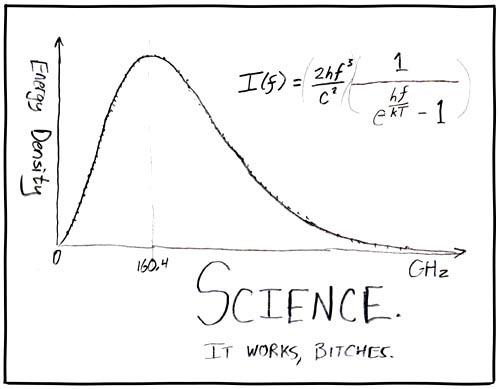
\includegraphics[width=.6\columnwidth]{science}
        \end{figure}
      \end{block}

      %-- Block 3-1
      \begin{block}{Experiments}
        Remember to put lots of figures on your poster... Nobody reads anymore!
      \end{block}

      %-- Block 3-2
      \begin{block}{Conclusion}
        Much less annoying than PowerPoint.  Copy and Paste from your
        document. Overall, a great idea!
      \end{block}

    \end{column}%2

% I think we should do just 2 columns
%     %-- Column 3 ---------------------------------------------------
%     \begin{column}{0.32\linewidth}
% 
%     \end{column}%3

  \end{columns}
\end{frame}
\end{document}
